\section{Results} \label{results}
\subsection{Encoding via VGG19}
The learning curve of the Autoencoder training is presented on Figure \ref{fig:vgg19_learning_curve}.
The initial high loss values are reduced significantly during the first few epochs.
The train and validation losses converge quite close to each other due to the fact that
the train dataset (as the overall dataset itself) contains mostly \emph{normal} rail images.
The validation curve is slightly above the train losses, there is no sign of overfitting or abnormal
training of the model.

\begin{figure}[!ht]
    \centering
    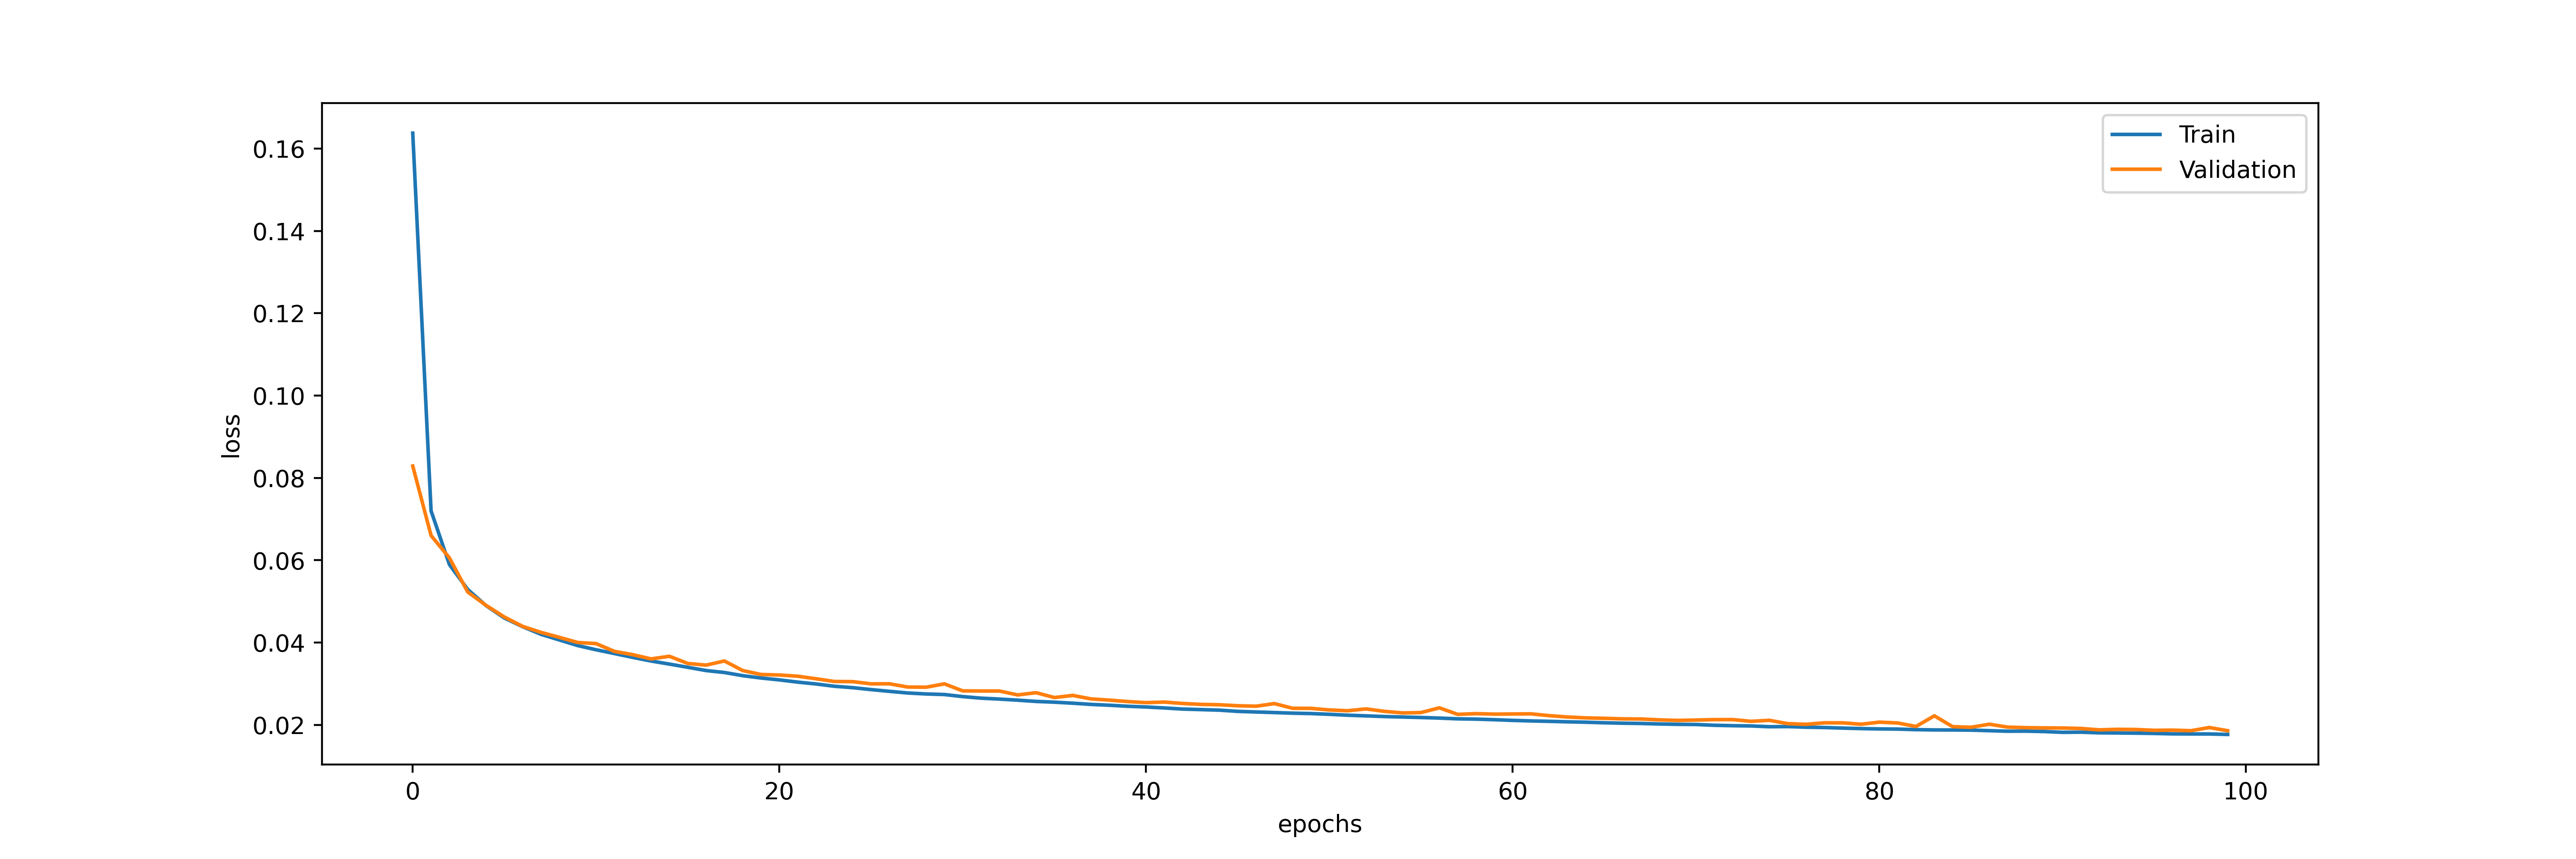
\includegraphics[width=\textwidth,trim={0 0 0 1cm},clip]{./results/vgg19_vgg19/20230510_172958_results.png}
    \caption{Learning curve of the VGG19 Encoder}
    \label{fig:vgg19_learning_curve}
\end{figure}

After training some example images are predicted (encoded and decoded) to visualise the performance
of the Autoencoder.
This is represented on Figure \ref{fig:vgg19_examples}.
The sample autoencoded images show the main characteristics that is recorded by the model.
The vertical shiny edge of the rail is easily identified.
The details that are close to the center of the image or are brighter parts of the image are
more likely to be captured.

\begin{figure}[!ht]
    \centering
    \begin{subfigure}{\textwidth}
        \centering
        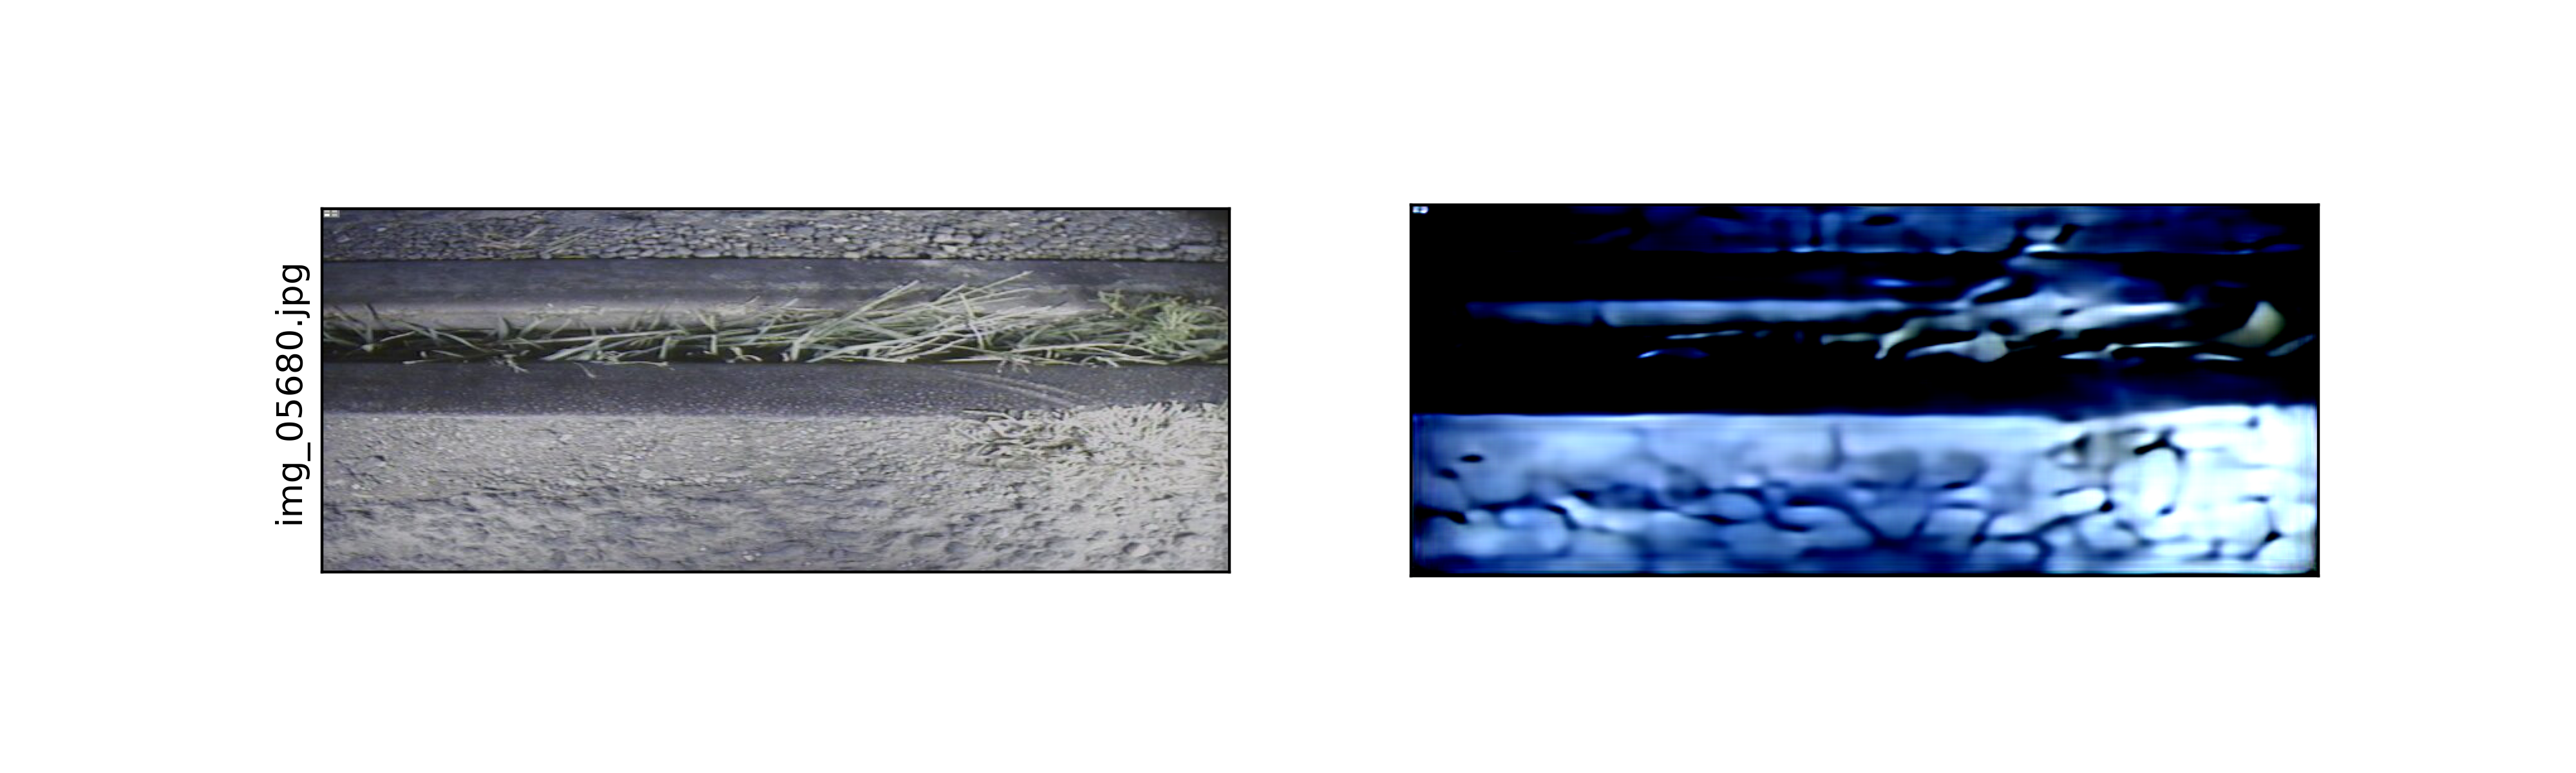
\includegraphics[width=0.9\textwidth,trim={0 1cm 0 1cm},clip]{./results/vgg19_vgg19/20230510_172958_predict_0.png}
    \end{subfigure}
    \begin{subfigure}{\textwidth}
        \centering
        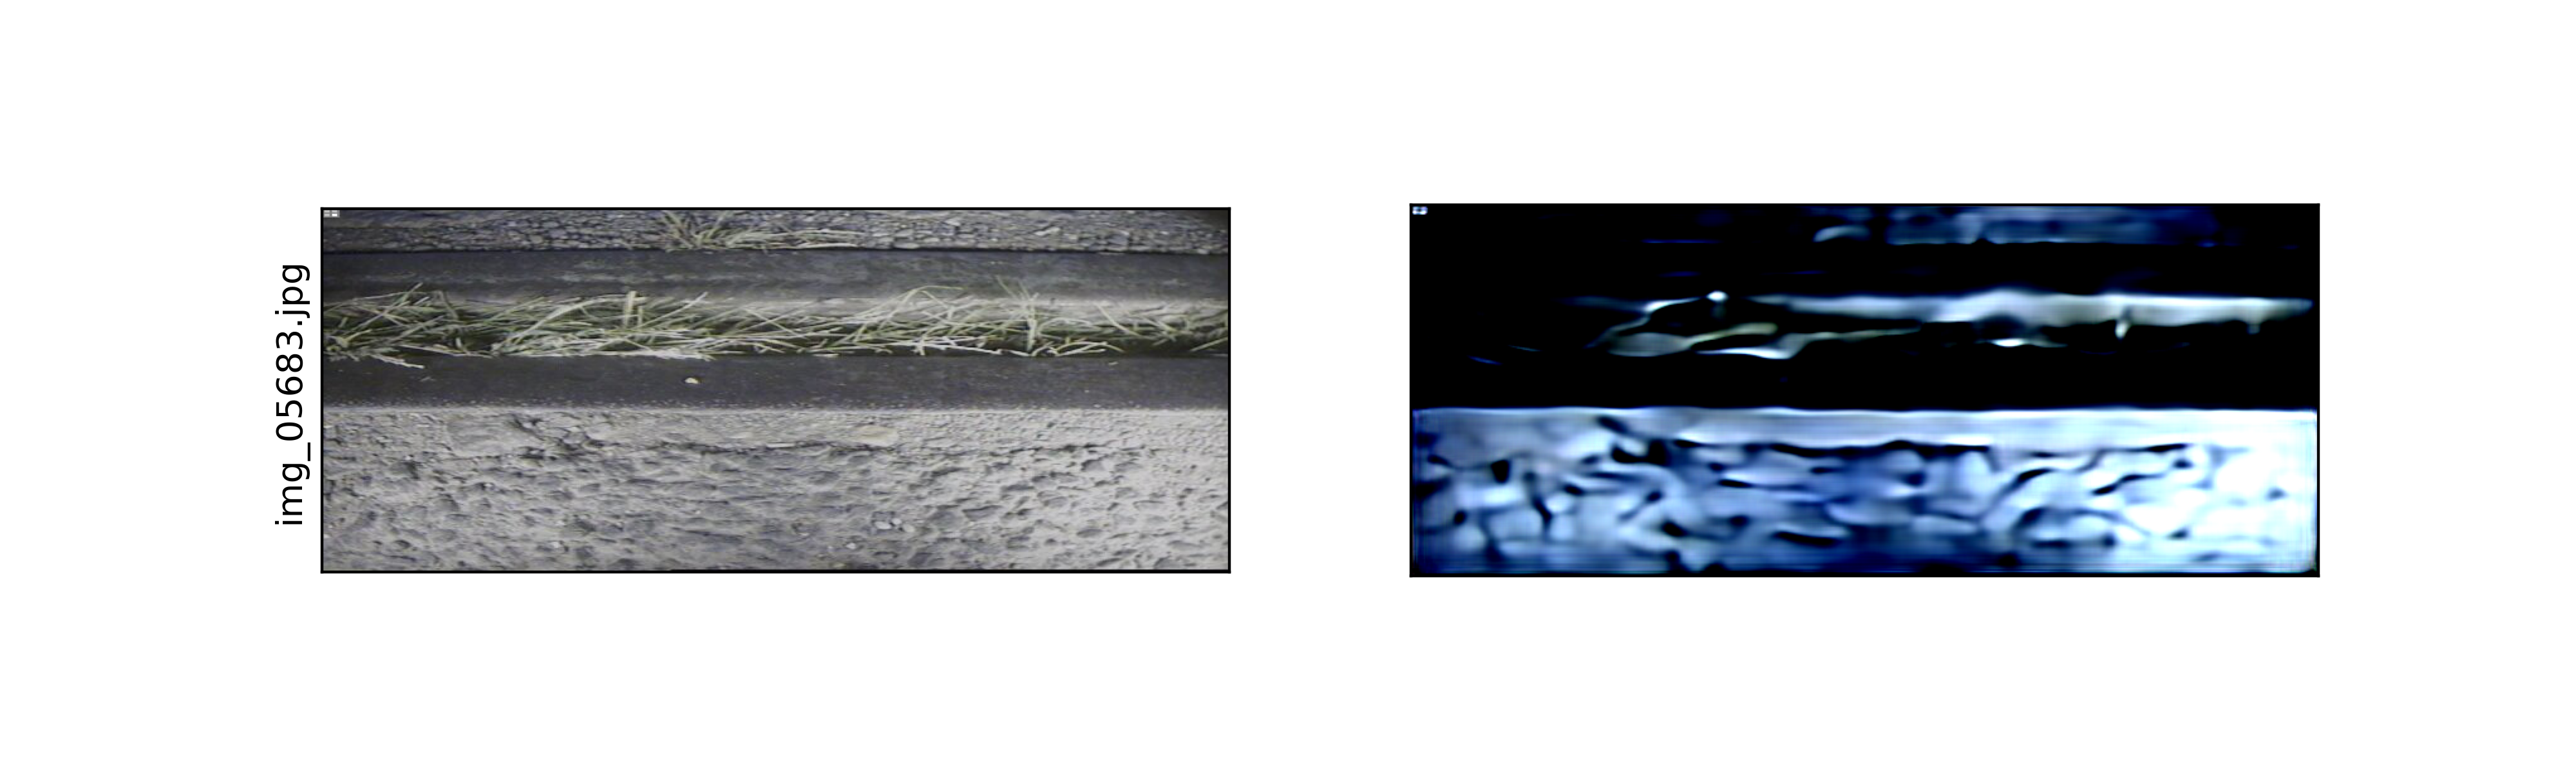
\includegraphics[width=0.9\textwidth,trim={0 1cm 0 1cm},clip]{./results/vgg19_vgg19/20230510_172958_predict_1.png}
    \end{subfigure}
    \begin{subfigure}{\textwidth}
        \centering
        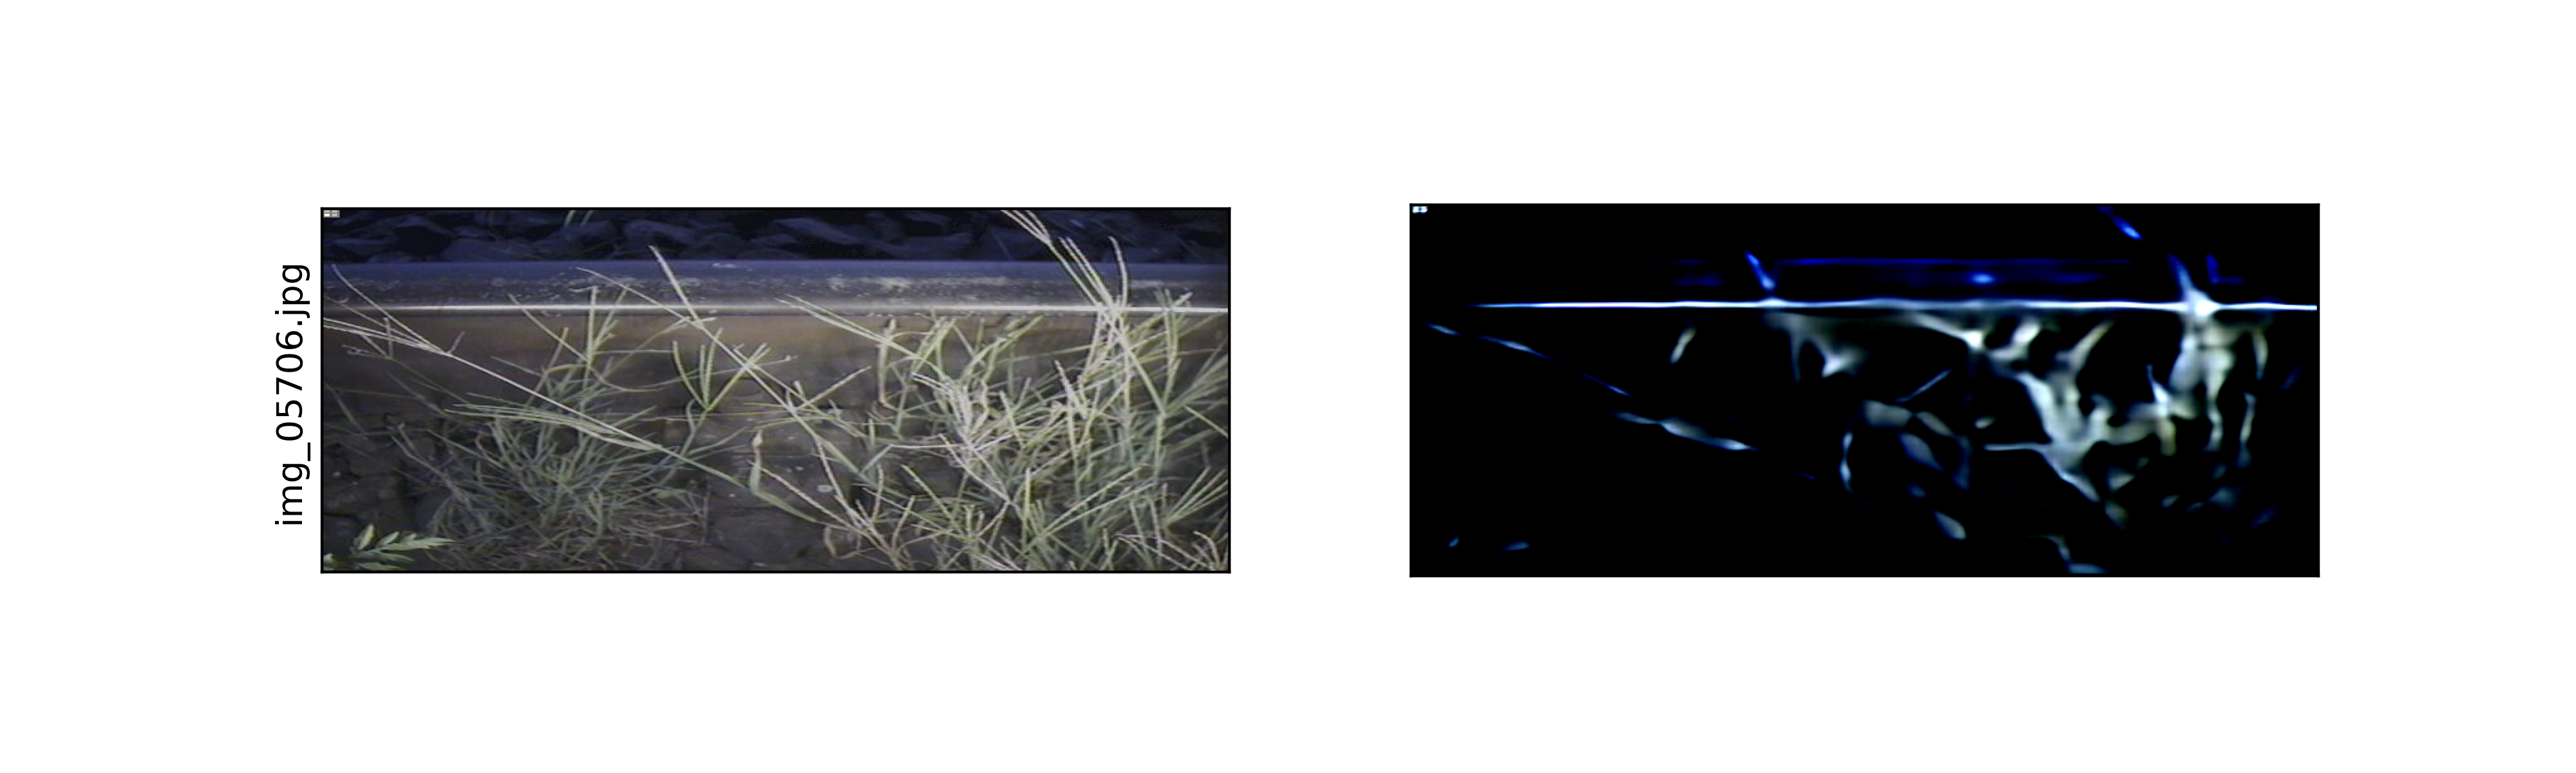
\includegraphics[width=0.9\textwidth,trim={0 1cm 0 1cm},clip]{./results/vgg19_vgg19/20230510_172958_predict_2.png}
    \end{subfigure}
    \caption{Predicted images in case of VGG19 Encoder}
    \label{fig:vgg19_examples}
\end{figure}

The visualization of the different model stages based on the PCA / t-SNE approach is depicted on
Figure \ref{fig:vgg19_pca}.
The colors indicate whether we observe a \emph{normal}, \emph{grass covered} or \emph{double rail}
image, the latter two is considered as outlier.
The alpha value of the markers indicate the loss value of the image, the higher the alpha
(less transparent) the marker is.
The outlier images form a certain cluster already among the input images, that is, at least to some
extent, retained after encoding.
This cluster are separated partially after encoding, there is a clear cluster made of the outliers,
but this cluster does not contain all members, some are still embedded among the \emph{normal} images,
however slightly moved to the boundary of it.
It can be also seen that after encoding these outliers are structured back to their original position
in the visualization space.
This indicates that the encoding is somehow clustering the dataset, whilst the decoding part readjust
this clustering back to it's origin, basically proving that the main idea of the Autoencoders is
represented in the model.

\begin{figure}[!ht]
    \centering
    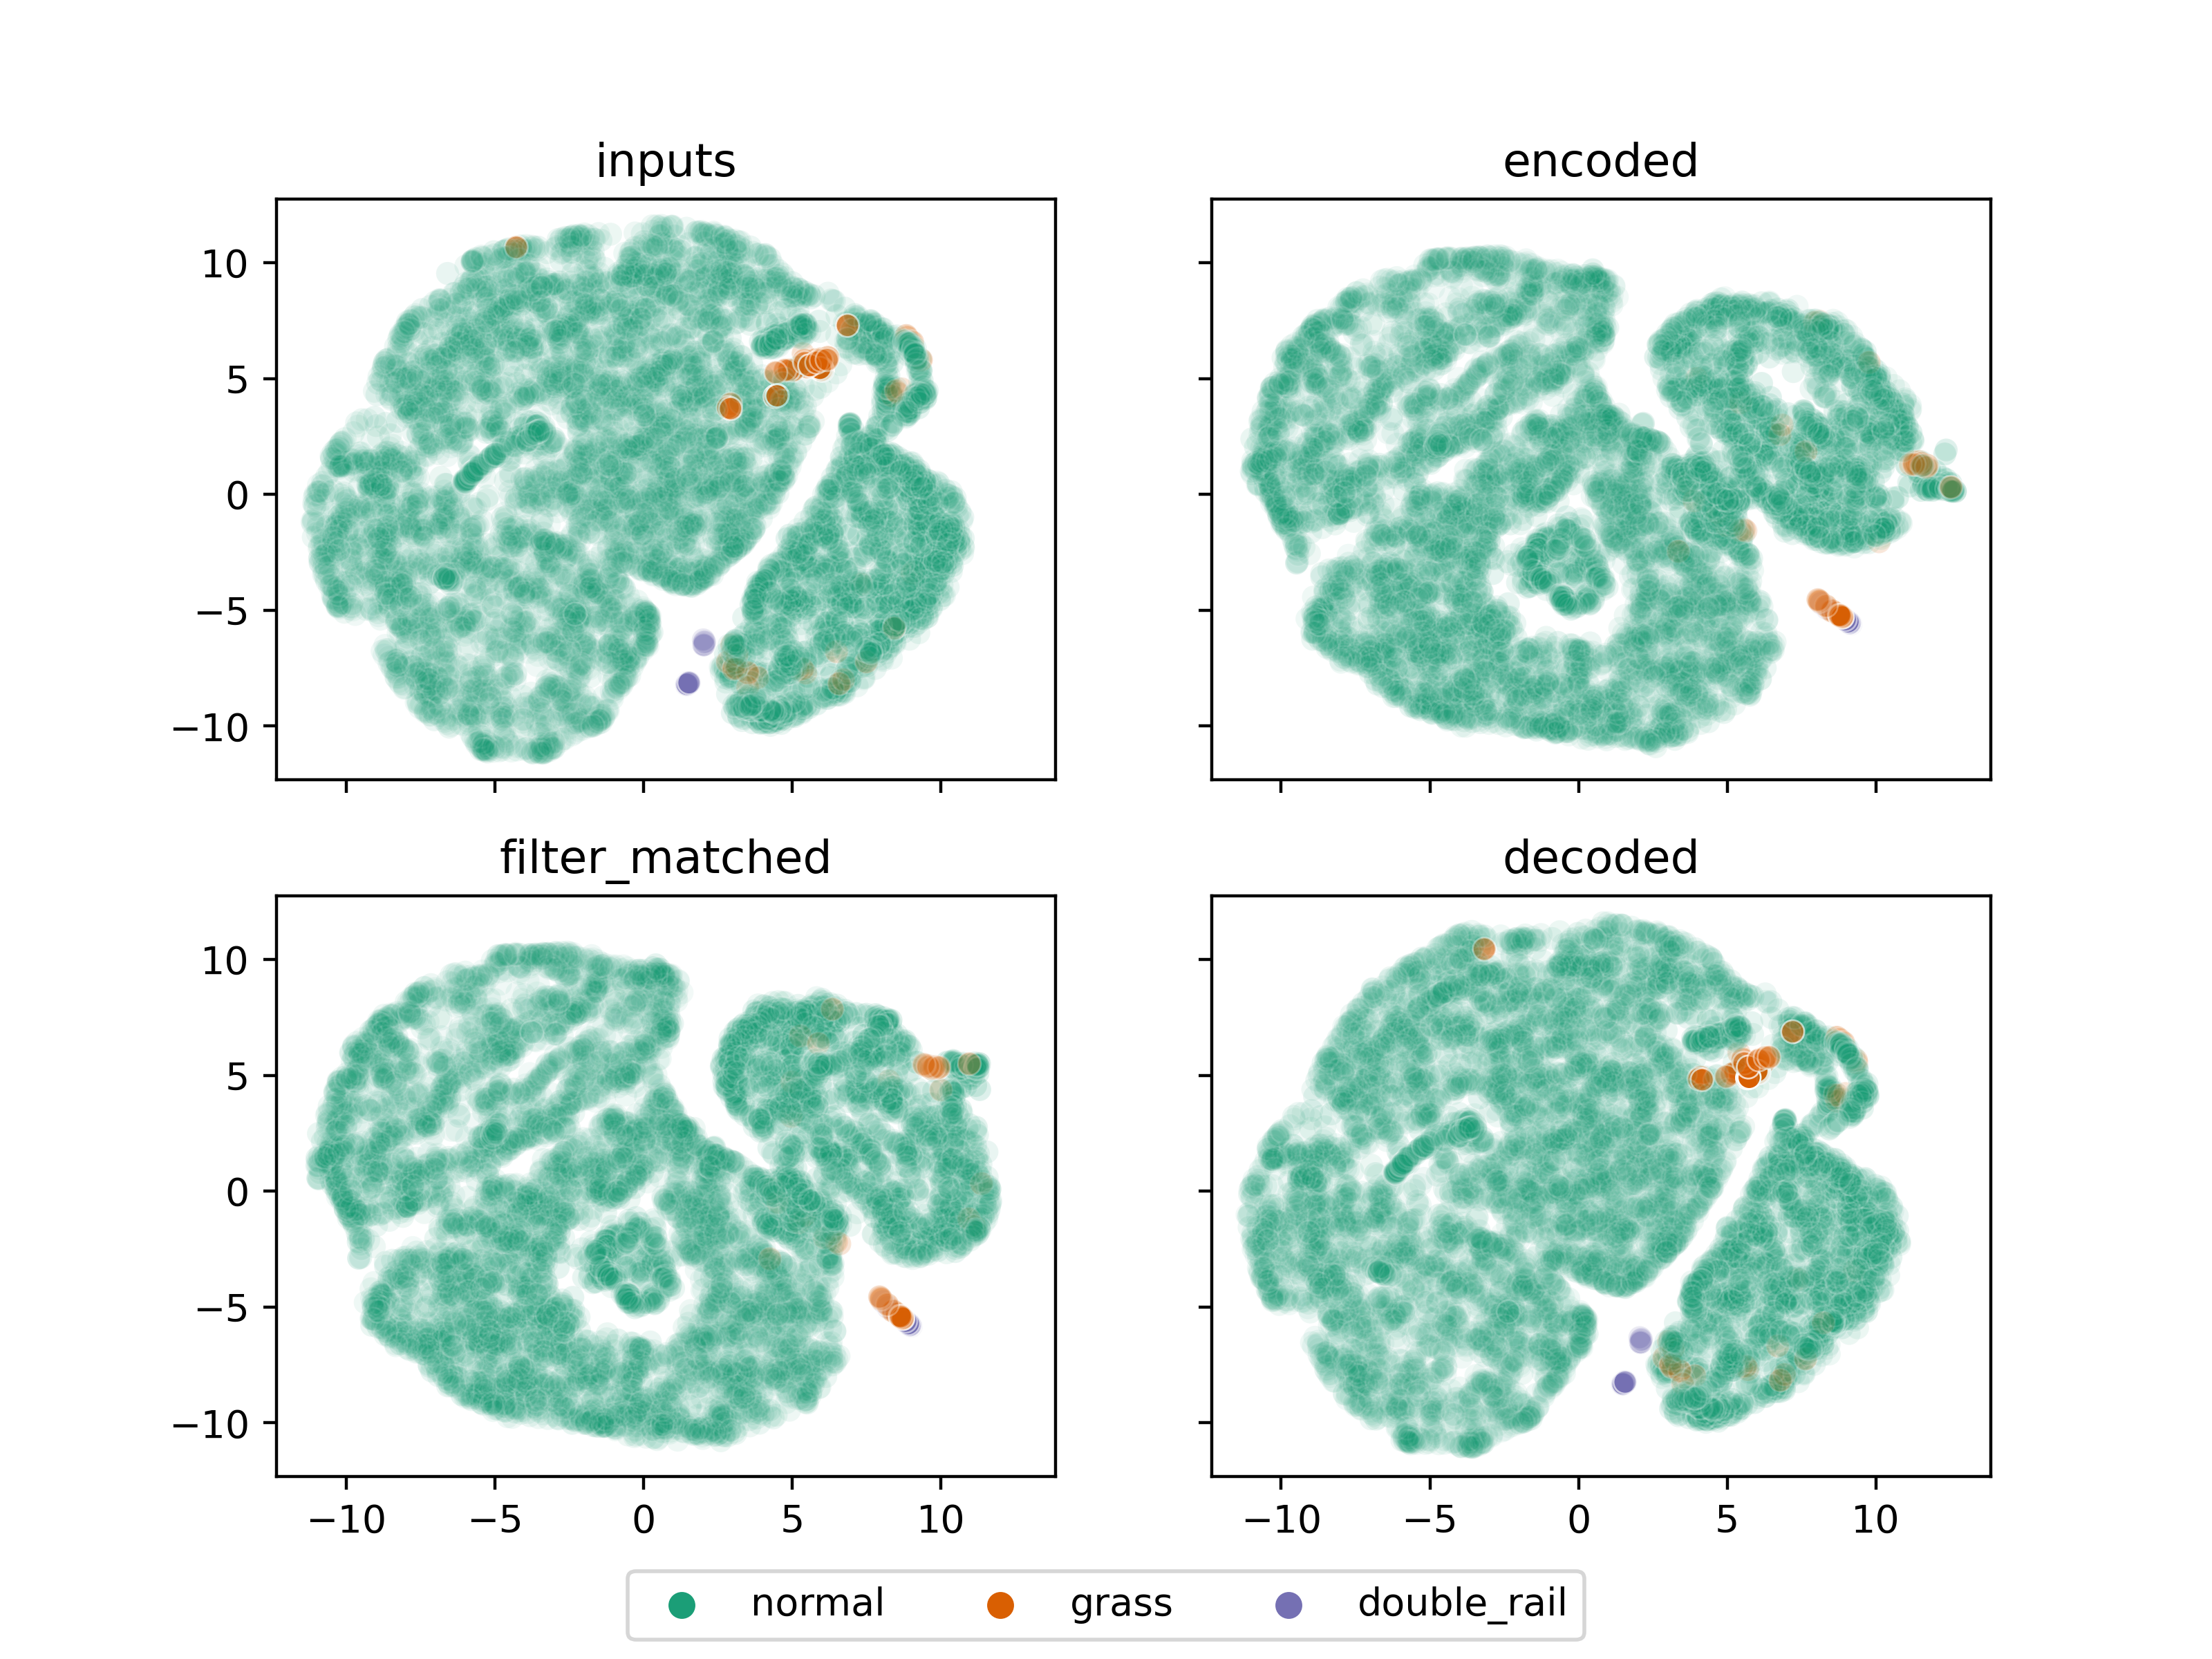
\includegraphics[width=\textwidth,trim={0 0 0 1cm},clip]{./results/vgg19_vgg19/20230510_172958_feature_vectors_1.png}
    \caption{PCA / t-SNE visualization of the VGG19 Encoder}
    \label{fig:vgg19_pca}
\end{figure}

The loss values of each image of the whole dataset together with a marking of the outliers is shown
on Figure \ref{fig:vgg19_loss}.
The peaks in the loss value are remarkably indicate the positions of the outlier images.
The concentration of the outliers are also confirmed based on the video footage, first a few seconds
of grass covered section can be seen, then in the second part a longer period of grass coverage
with the appearance of the double rails is present in the video.
It is to be noted that, for example in case of the first \emph{grass} image the loss value is not
so well distinguishes the image from it's neighbouring images.
Similarly, but in the opposite direction, at some \emph{normal} pictures the loss value is significantly
higher then the preceeding or following images.

\begin{figure}[!ht]
    \centering
    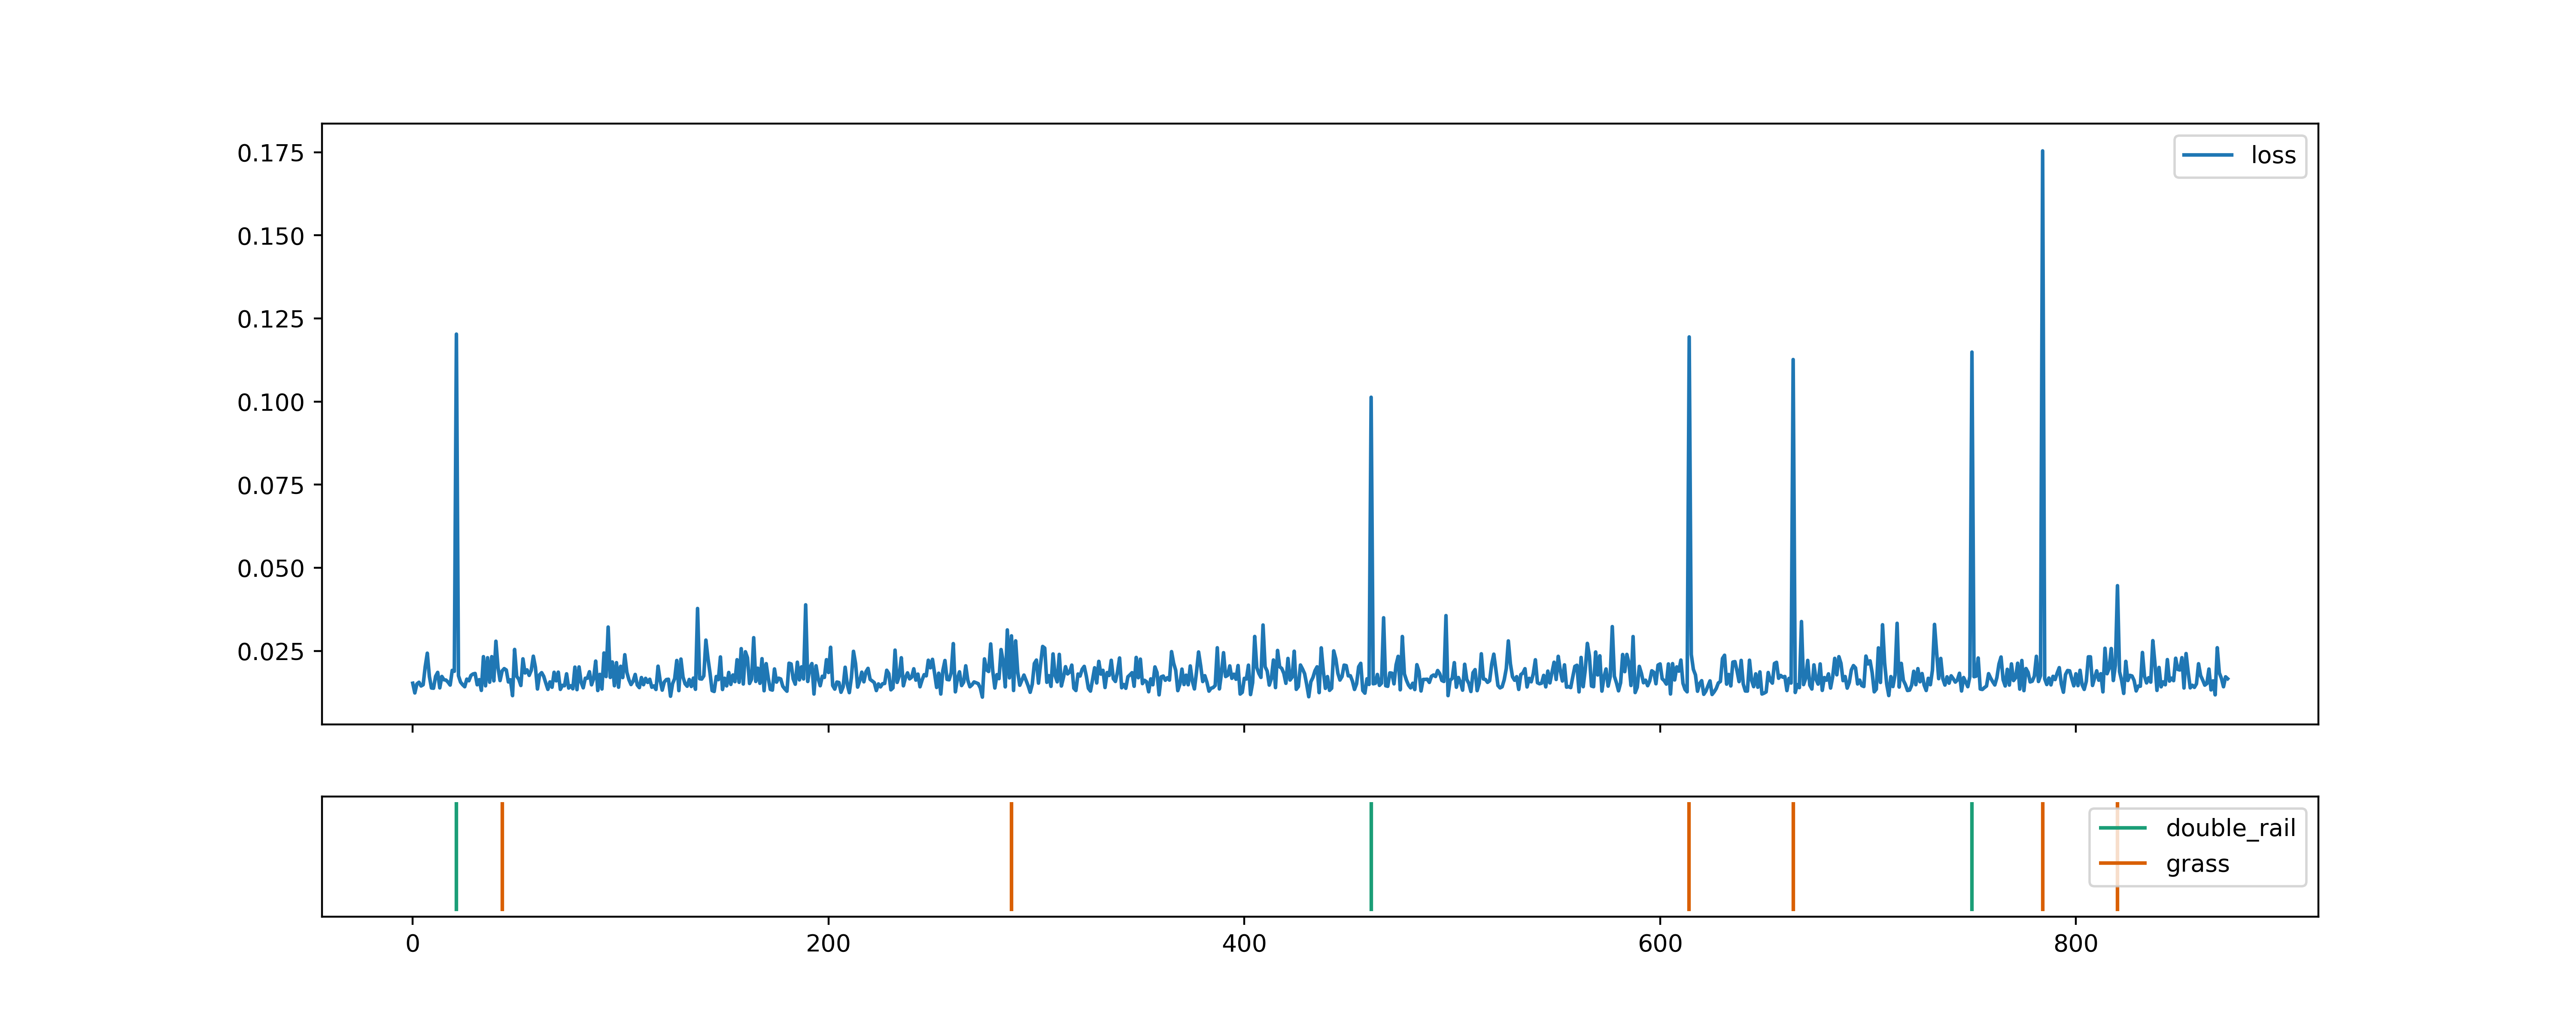
\includegraphics[width=\textwidth]{./results/vgg19_vgg19/20230510_172958_feature_vectors_loss.png}
    \caption{Loss values of the dataset with VGG19 encoding}
    \label{fig:vgg19_loss}
\end{figure}

The confusion matrix for the loss-based and Isolation Forest anomaly detection techniques can be seen
on Figure \ref{fig:vgg19_cm}.
The loss-based approach identifies the $\frac{2}{3}$ of the outliers correclty,
whilst providing no false positive.
The threshold of three times the standard deviations seems to be a quite conservative approach,
considering the actual use case that the target is to identify all the outliers, even with the cost
of increasing the false positive rate, lowering this threshold might be useful.
The Isolation Forest gives slightly different results, finding approximately half of the outliers,
and providing some number of false positives.

\begin{figure}[!ht]
    \centering
    \begin{subfigure}{0.4\textwidth}
        \centering
        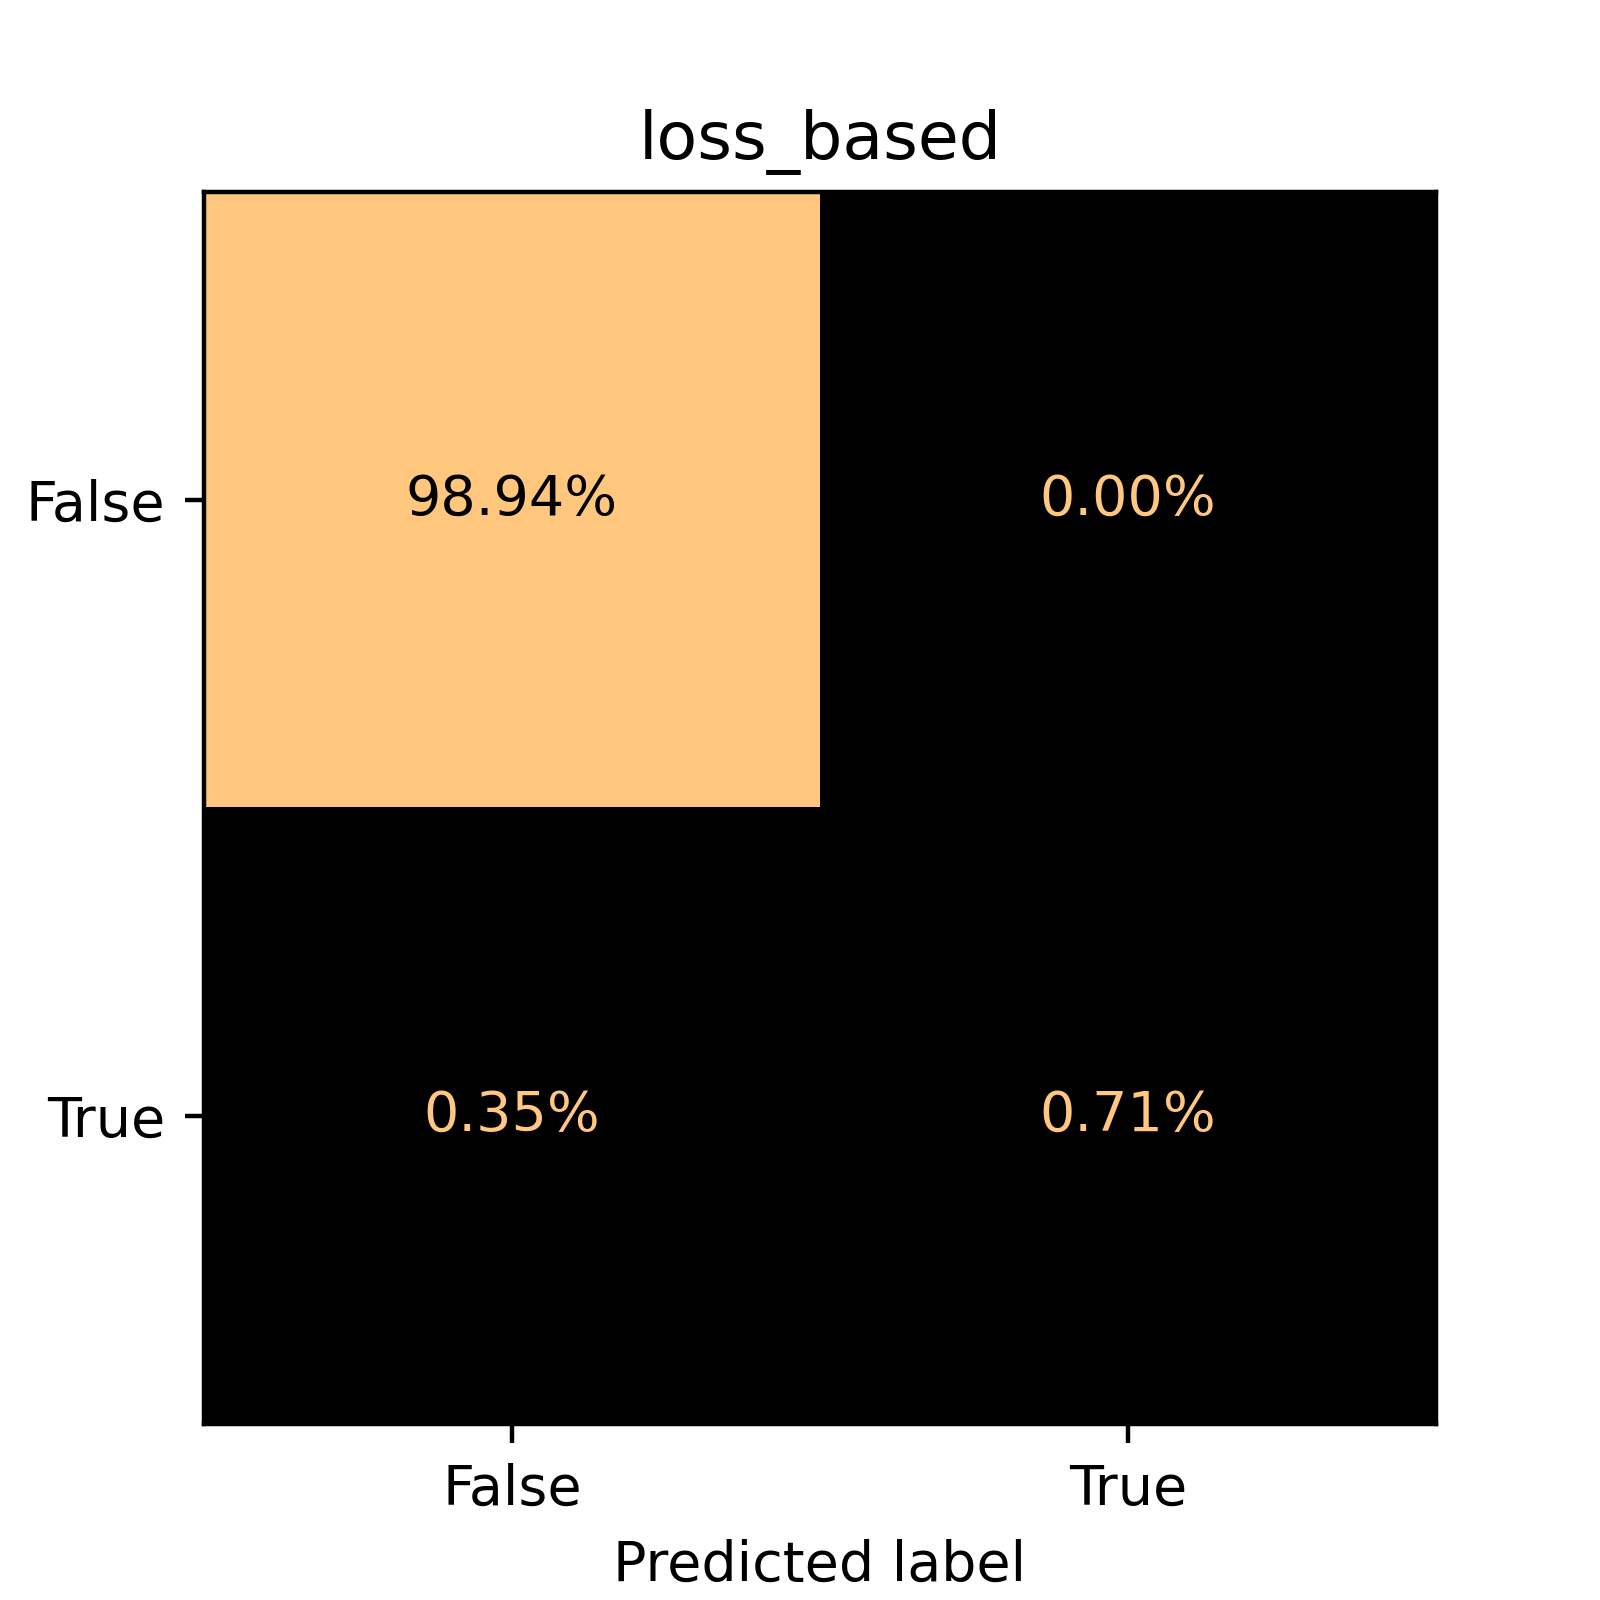
\includegraphics[width=\textwidth]{./results/vgg19_vgg19/20230510_172958_loss_based_cm.png}
    \end{subfigure}
    \begin{subfigure}{0.4\textwidth}
        \centering
        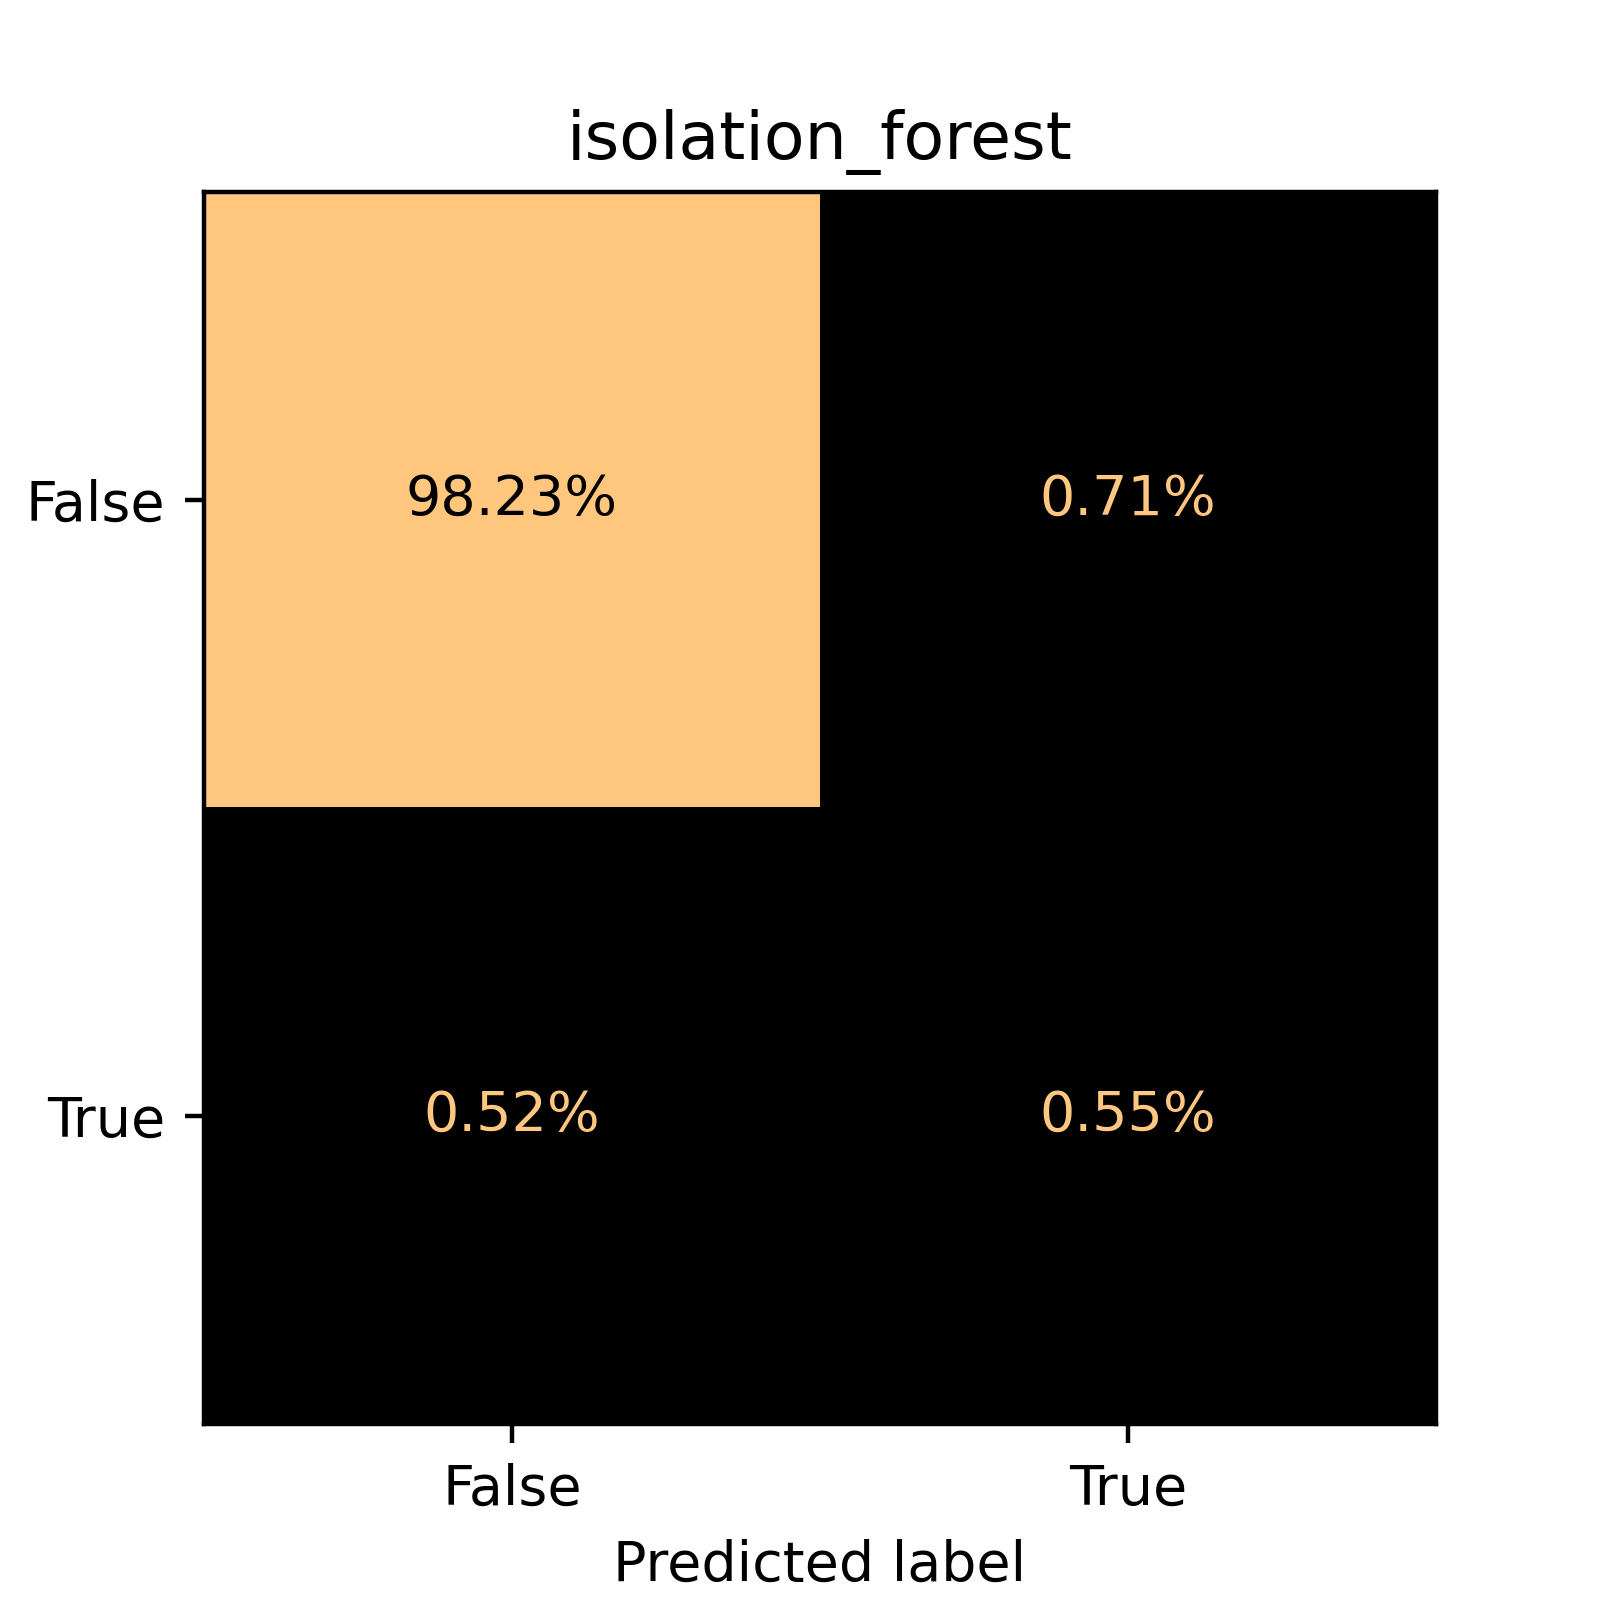
\includegraphics[width=\textwidth]{./results/vgg19_vgg19/20230510_172958_isolation_forest_cm.png}
    \end{subfigure}
    \caption{Confusion Matrices of the VGG19 encoder}
    \label{fig:vgg19_cm}
\end{figure}